\documentclass[tikz,border=0pt]{standalone}
\usepackage[american]{circuitikz}
\usetikzlibrary{arrows.meta,calc,positioning,decorations.pathmorphing,patterns}
\definecolor{zyloTeal}{HTML}{174A5B}
\definecolor{zyloTealTwo}{HTML}{246B7A}
\definecolor{zyloInk}{HTML}{1F2933}
\definecolor{zyloSoft}{HTML}{EAF4F4}
\definecolor{zyloPaper}{HTML}{F8FAFB}
\definecolor{zyloLine}{HTML}{44606B}
\definecolor{zyloOrange}{HTML}{D97706}
\begin{document}
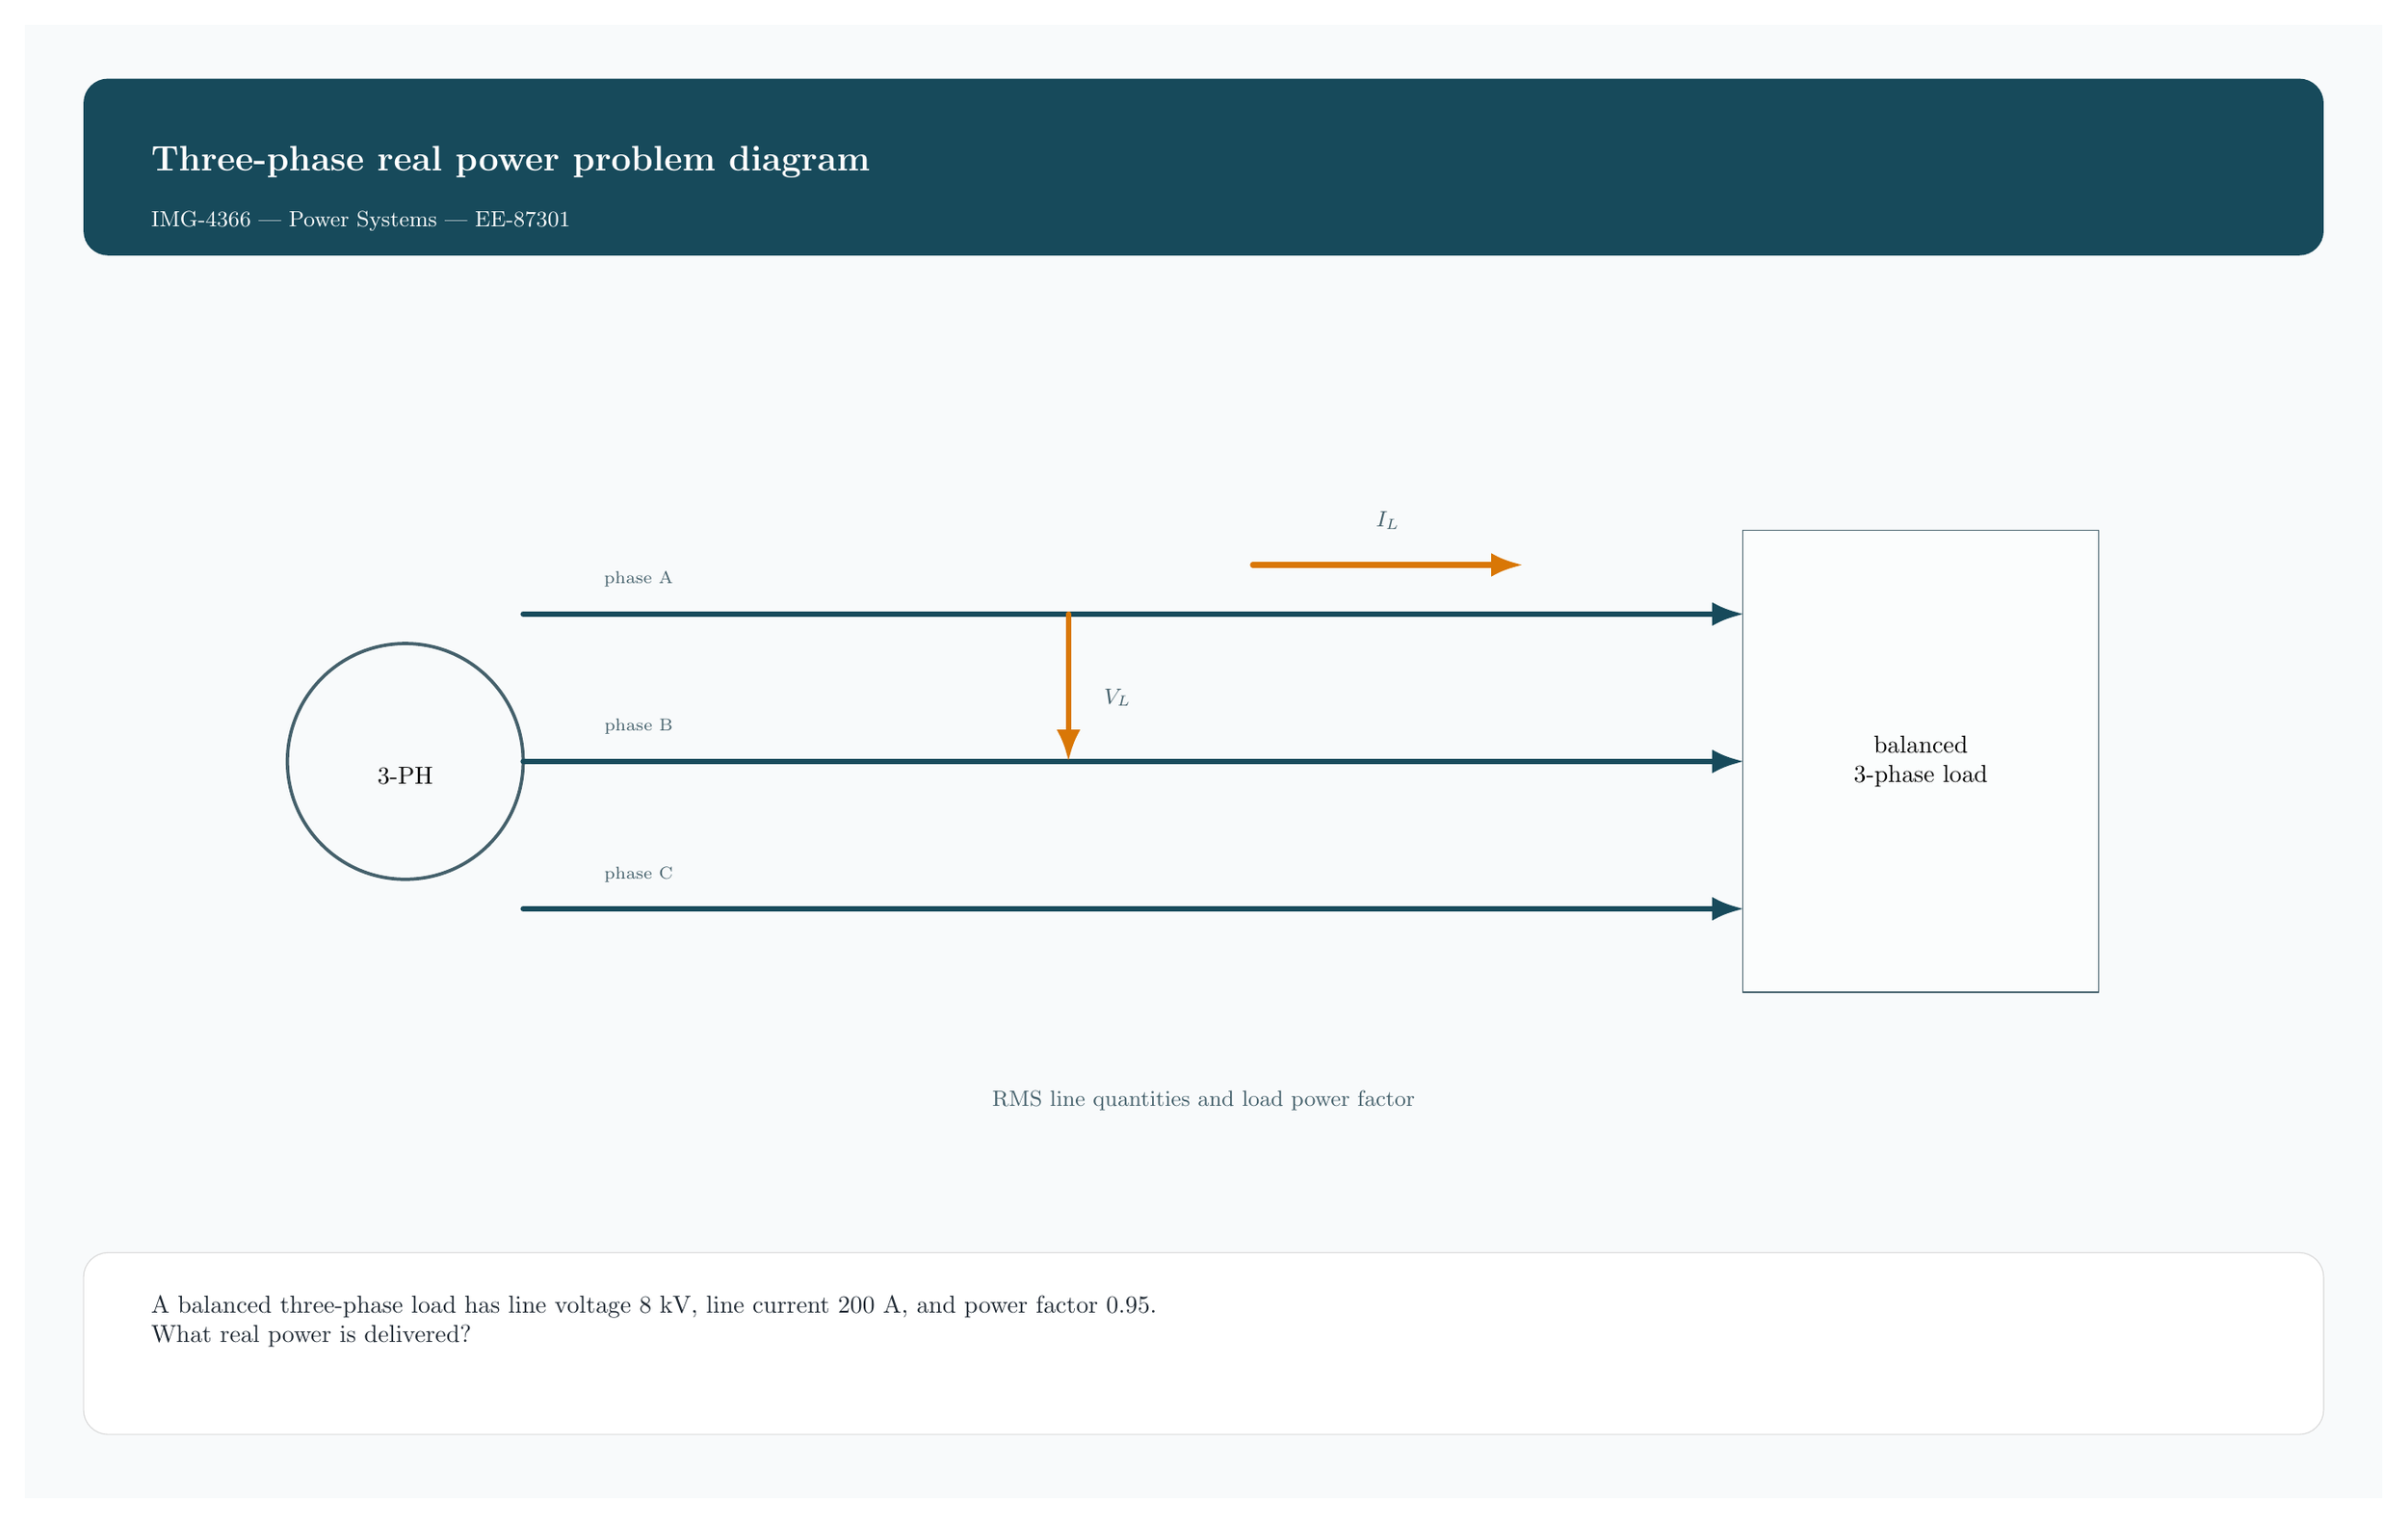
\begin{tikzpicture}[x=1pt,y=-1pt,>=Latex,line cap=round,line join=round]
\path[fill=zyloPaper] (0,0) rectangle (960,600);
\path[fill=zyloTeal,rounded corners=10pt] (24,22) rectangle (936,94);
\node[anchor=west,text=white,font=\bfseries\Large] at (48,56) {Three-phase real power problem diagram};
\node[anchor=west,text=white!82,font=\small] at (48,80) {IMG-4366 | Power Systems | EE-87301};
\tikzset{wire/.style={draw=zyloTeal,line width=2.2pt},thinwire/.style={draw=zyloLine,line width=1.35pt},accent/.style={draw=zyloOrange,line width=2.2pt},box/.style={draw=zyloTealTwo,fill=zyloSoft,line width=1.5pt,rounded corners=8pt}}
\draw[thinwire] (155,300) circle (48); \node at (155,306) {3-PH};
\draw[wire,->] (203,240) -- (700,240); \draw[wire,->] (203,300) -- (700,300); \draw[wire,->] (203,360) -- (700,360);
\node[font=\scriptsize,text=zyloLine] at (250,226) {phase A}; \node[font=\scriptsize,text=zyloLine] at (250,286) {phase B}; \node[font=\scriptsize,text=zyloLine] at (250,346) {phase C};
\node[draw=zyloLine,fill=white!80!zyloSoft,minimum width=145pt,minimum height=188pt,align=center] at (772,300) {balanced\\3-phase load};
\draw[accent,->] (425,240) -- (425,300); \node[font=\small,text=zyloLine] at (445,274) {$V_L$};
\draw[accent,->] (500,220) -- (610,220); \node[font=\small,text=zyloLine] at (555,202) {$I_L$};
\node[font=\small,text=zyloLine] at (480,438) {RMS line quantities and load power factor};
\path[draw=black!15,fill=white,rounded corners=10pt] (24,500) rectangle (936,574);
\node[anchor=west,text width=860pt,align=left,text=zyloInk,font=\normalsize] at (48,528) {A balanced three-phase load has line voltage 8 kV, line current 200 A, and power factor 0.95.\\What real power is delivered?};
\end{tikzpicture}
\end{document}
